\documentclass[a4paper]{article}
\usepackage{ctex}
\usepackage{enumitem}
\usepackage{fancyhdr}
\usepackage{amsmath}
\usepackage{parskip}
\usepackage{float}
\usepackage{listings}
\usepackage{hyperref}
\usepackage{xcolor}
\usepackage{pgf}
\usepackage{tikz}

\usetikzlibrary{arrows,automata}

\setlength{\parskip}{6pt}

\pagestyle{headings}

\begin{document}
\title{串行密码锁}
\author{梁业升 2019010547(计03)}

\maketitle

% GitHub styles
\definecolor{keyword}{HTML}{CF222E}
\definecolor{comment}{HTML}{6E7781}
\definecolor{string}{HTML}{0A3069}

\lstset{
    commentstyle=\color{comment},
    keywordstyle=\color{keyword},
    stringstyle=\color{string},
    basicstyle=\ttfamily\small,
    breakatwhitespace=false,
    breaklines=true,
    captionpos=b,
    keepspaces=true,
    showspaces=false,
    showstringspaces=false,
    showtabs=false,
}


\section{实现}

\begin{lstlisting}[language=vhdl]
library ieee;
use ieee.std_logic_1164.all;
use ieee.std_logic_arith.all;
use ieee.std_logic_unsigned.all;

entity lock is
    port(
        rst, clk: in std_logic;
        mode: in std_logic_vector(1 downto 0);
        code: in std_logic_vector(3 downto 0);
        unlocked, err, locked, warn: out std_logic
    );
end lock;

architecture arch of lock is
    signal state: integer := -1;
    signal err_cnt: integer := 0;
    signal pass0, pass1, pass2, pass3: std_logic_vector(3 downto 0);
begin
    process(clk, rst)
    begin
        if (rst = '1') then
            if (state = -1) then -- ready to set
                state <= 0;
            elsif (state = -2) then -- ready to unlock
                state <= 4;
            elsif (state = -3) then -- admin
                state <= 8;
            end if;
            err <= '0';
            unlocked <= '0';
            if (err_cnt < 3) then
                warn <= '0';
            end if;
        elsif (rising_edge(clk)) then
            if (state >= 0) then -- valid
                if (mode = "00") then -- set passwd
                    case state is
                        when 0 =>
                            pass0 <= code;
                            state <= 1;
                        when 1 =>
                            pass1 <= code;
                            state <= 2;
                        when 2 =>
                            pass2 <= code;
                            state <= 3;
                        when 3 =>
                            pass3 <= code;
                            state <= -2; -- set successfully
                            locked <= '1';
                        when others => null; -- wrong mode
                    end case;
                elsif (mode = "01") then -- input passwd
                    case state is
                        when 4 =>
                            if (code = pass0) then
                                state <= 5;
                            else
                                state <= -2;
                                err <= '1';
                                if (err_cnt >= 2) then
                                    warn <= '1';
                                    state <= -3; -- admin mode
                                end if;
                                err_cnt <= err_cnt + 1;
                            end if;
                        when 5 =>
                            if (code = pass1) then
                                state <= 6;
                            else
                                state <= -2;
                                err <= '1';
                                if (err_cnt >= 2) then
                                    warn <= '1';
                                    state <= -3; -- admin mode
                                end if;
                                err_cnt <= err_cnt + 1;
                            end if;
                        when 6 =>
                            if (code = pass2) then
                                state <= 7;
                            else
                                state <= -2;
                                err <= '1';
                                if (err_cnt >= 2) then
                                    warn <= '1';
                                    state <= -3; -- admin mode
                                end if;
                                err_cnt <= err_cnt + 1;
                            end if;
                        when 7 =>
                            if (code = pass3) then
                                state <= -1; -- success
                                unlocked <= '1';
                                locked <= '0';
                                err_cnt <= 0; -- reset err_cnt
                            else
                                state <= -2;
                                err <= '1';
                                if (err_cnt >= 2) then
                                    warn <= '1';
                                    state <= -3; -- admin mode
                                end if;
                                err_cnt <= err_cnt + 1;
                            end if;
                        when others => null; -- wrong mode
                    end case;
                elsif (mode = "11") then -- admin
                    case state is
                        when 8 =>
                            if (code = "1000") then
                                state <= 9;
                            else
                                state <= -3;
                                err <= '1';
                            end if;
                        when 9 =>
                            if (code = "0100") then
                                state <= 10;
                            else
                                state <= -3;
                                err <= '1';
                            end if;
                        when 10 =>
                            if (code = "0010") then
                                state <= 11;
                            else
                                state <= -3;
                                err <= '1';
                            end if;
                        when 11 =>
                            if (code = "0001") then
                                state <= -1; -- success
                                unlocked <= '1';
                                locked <= '0';
                                err_cnt <= 0; -- reset err_cnt
                            else
                                state <= -3;
                                err <= '1';
                            end if;
                        when others => null; -- wrong mode
                    end case;
                end if;
            end if;
        end if;
    end process;
    
end arch;
\end{lstlisting}

输入和输出除了课本的要求外额外增加了一个 \texttt{locked} 用于指示当前密码锁是否已上锁。

状态机(不包含密码预置和系统报警)如下:

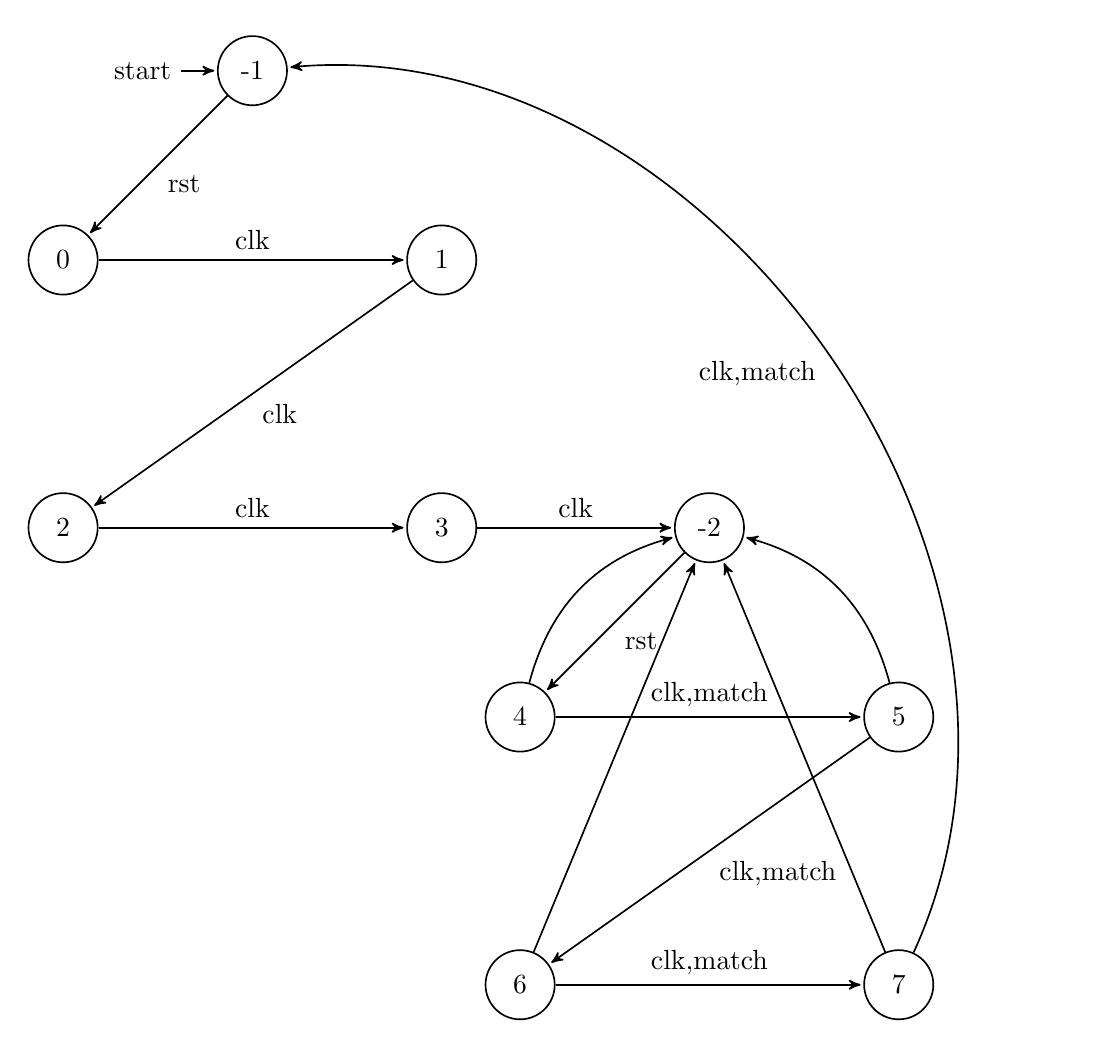
\begin{tikzpicture}[->,>=stealth',shorten >=1pt,auto,node distance=3.4cm,
    semithick]

\node[initial,state] (start)                        {-1};
\node[state]         (0) [below left of=start] {0};
\node[state]         (1) [below right of=start] {1};
\node[state]         (2) [below of=0] {2};
\node[state]         (3) [below of=1] {3};

\node[state]         (start-2) [right of=3] {-2};
\node[state]         (4) [below left of=start-2] {4};
\node[state]         (5) [below right of=start-2] {5};
\node[state]         (6) [below of=4] {6};
\node[state]         (7) [below of=5] {7};


\path (start) edge node {rst} (0);
\path (0) edge node {clk} (1);
\path (1) edge node {clk} (2);
\path (2) edge node {clk} (3);

\path (3) edge node {clk} (start-2);
\path (start-2) edge node {rst} (4);
\path (4) edge node {clk,match} (5);
\path (5) edge node {clk,match} (6);
\path (6) edge node {clk,match} (7);
\path (4) edge [bend left] node {} (start-2);
\path (5) edge [bend right] node {} (start-2);
\path (6) edge node {} (start-2);
\path (7) edge node {} (start-2);
\path (7) edge [bend right=60] node {clk,match} (start);

\end{tikzpicture}

上面状态 -2 至 7 与代码中 \texttt{state} 的值对应,其中:

\begin{itemize}
    \item -1 表示待进行密码的设置。
    \item 0 至 3 分别表示第 1 至 4 位密码的设置。
    \item -2 表示待进行密码的输入。
    \item 4 至 7 分别表示第 1 至 4 位密码的验证,若匹配,进入下一个状态;若不匹配,回到状态 2。状态 7 密码输入正确后返回初始状态 -1。
\end{itemize}

另外,状态 -3 以及 8 至 12 对应管理员模式,状态机与密码输入模式类似,在上图中未画出。

\section{仿真}

仿真结果如下:

\begin{figure}[H]
    \centering
    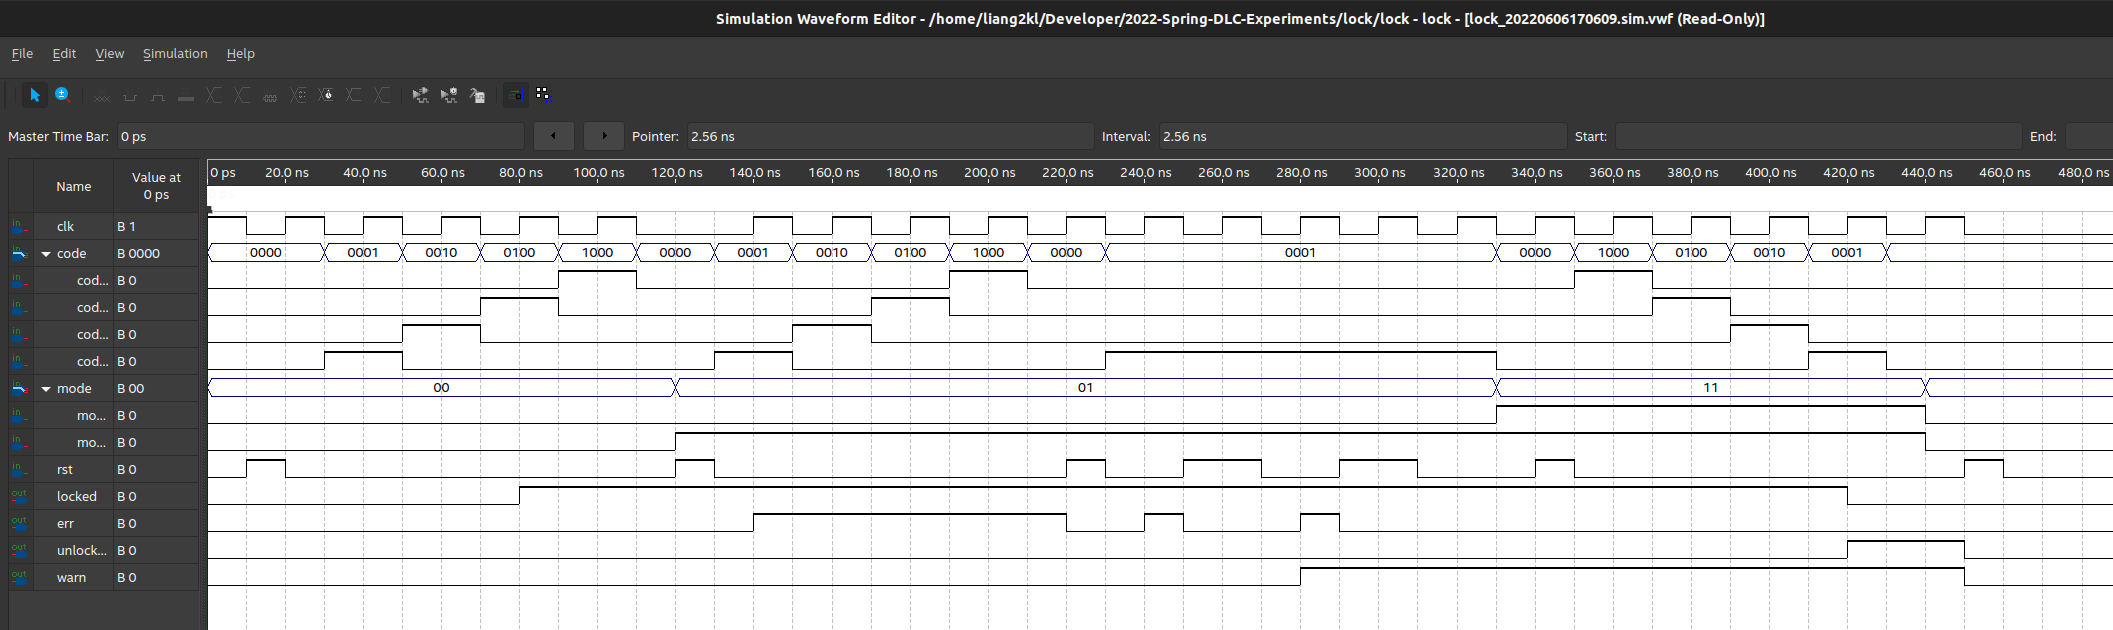
\includegraphics[width=1\textwidth]{./assets/simulation.png}
\end{figure}

首先进行密码的设置;然后选择输入密码的模式,首先输入正确的密码,可以看到成功解锁;然后重新设置密码,并输入
错误的密码,可以看到三次错误后发出报警。这时我们切换到管理员模式,使用预设的密码,可以看到成功解锁。

\section{总结}

本次是最后一次 CPLD 实验,相比于前几次的实验,本次实验代码编写和仿真进展比较顺利,可见经过几次实验的训练后对 VHDL 已经比较熟练了。这次实验也是第一次使用状态机进行设计,状态机的方法具有清晰、直观的特点,适合用于状态较为复杂的电路的设计。

\end{document}
